% BHU PYQ -- Professional Exam Template
\documentclass[11pt,a4paper]{article}

\usepackage[a4paper,top=2.5cm,bottom=2.5cm,left=2.8cm,right=2.8cm,headheight=14pt]{geometry}
\usepackage{amsmath,amssymb}
\usepackage[T1]{fontenc}
\usepackage[utf8]{inputenc}
\usepackage{lmodern}
\usepackage{microtype}
\usepackage{fancyhdr}
\usepackage{enumitem}
\usepackage{hyperref}
\usepackage{lastpage}
\usepackage{parskip}
\usepackage{tikz}
\usetikzlibrary{arrows.meta,shapes,positioning}

\hypersetup{colorlinks=true,urlcolor=black,linkcolor=black,
  pdftitle={B.Sc. (Hons.) Zoology Sem-I ZOB-101 -- BHU PYQ}}

\pagestyle{fancy}
\fancyhf{}
\renewcommand{\headrulewidth}{0.4pt}
\renewcommand{\footrulewidth}{0.4pt}
\fancyhead[L]{\small   \textit{Banaras Hindu University}}
\fancyhead[R]{\small   \textit{Zoology Paper: ZOB-101}}
\fancyfoot[C]{\small Page  \thepage\ of \pageref{LastPage}}


\newlist{parts}{enumerate}{2}
\setlist[parts,1]{label=(\alph*),leftmargin=*,itemsep=4pt,topsep=3pt}
\setlist[parts,2]{label=(\roman*),leftmargin=*,itemsep=2pt,topsep=2pt}

\newcommand{\pts}[1]{\hfill   \textit{[#1]}}


\begin{document}


\begin{center}
  {\large\bfseries BANARAS HINDU UNIVERSITY}\\[2pt]
  {
\normalsize B.Sc. (Hons.) Semester I Examination, 2022-23}\\[6pt]
  \rule{0.8\linewidth}{0.5pt}\\[6pt]
  {\large\bfseries Zoology}\\[4pt]
  {\large\bfseries Paper: ZOB-101 --- Animal Diversity and Animal Form and Function}\\[4pt]
  {
\normalsize Time: Three hours \hfill Full Marks: 70}
\end{center}

\rule{\linewidth}{0.4pt}

\smallskip



\noindent   \textit{Note: Answer three questions from Section-A and three questions from Section-B. Question No. 1 in both sections is compulsory. Use a separate answer book for each section. The figures in the right-hand margin indicate marks.}

\bigskip

\begin{center}
   \textbf{SECTION -- A} \\
   \textbf{(Animal Diversity) (Marks: 35)}
\end{center}

\medskip


\noindent   \textbf{Question 1.} Answer the following parts:

\begin{parts}
  \item State whether the following statements are True or False. Justify your answer in 2-3 sentences each:\pts{$2  \times 4 = 8$}
  
\begin{parts}
    \item Animals that display radial symmetry are triploblastic.
    \item Development in deuterostomes is marked by radial cleavage and enterocoely.
    \item Cyclostomes are acraniates with paired fins and a bony skeleton.
    \item All chordates are vertebrates but all vertebrates are not chordates.
  \end{parts}
  \item Define cloacal respiration.\pts{1}
  \item Differentiate between neoteny and pedogenesis.\pts{2}
\end{parts}

\medskip


\noindent   \textbf{Question 2.} Answer the following parts:

\begin{parts}
  \item Classify phylum   \textit{Cnidaria}   \textbf{OR}   \textit{Echinodermata} up to classes, giving characteristic features and suitable examples of each class.\pts{6}
  \item Discuss the general characters of   \textit{Hemichordata} and enumerate its various classes with suitable examples.\pts{6}
\end{parts}

\medskip


\noindent   \textbf{Question 3.} Answer the following parts:

\begin{parts}
  \item Describe the salient features of class   \textit{Amphibia}   \textbf{OR}   \textit{Reptilia} and classify it up to orders, giving characteristic features with suitable examples.\pts{6}
  \item Explain some of the advantages brought about through the evolution of bilateral symmetry and coelom formation.\pts{6}
\end{parts}

\medskip


\noindent   \textbf{Question 4.} Write short notes on any two of the following:\pts{$6  \times 2 = 12$}

\begin{parts}
  \item Chelicerates
  \item Cetaceans
  \item Canal system of Poriferans
  \item Mosaic cleavage
\end{parts}

\pagebreak

\begin{center}
   \textbf{SECTION -- B} \\
   \textbf{(Animal Form and Function) (Marks: 35)}
\end{center}

\medskip


\noindent   \textbf{Question 1.} Answer the following parts:

\begin{parts}
  \item State whether the following statements are True or False. Justify your answer in 2-3 sentences each:\pts{$2  \times 4 = 8$}
  
\begin{parts}
    \item Apposition image is formed in nocturnal insects.
    \item Strobilation is a special type of transverse fission.
    \item Amphibians use a negative pressure pump mechanism for ventilating their lungs.
    \item Crocodiles have two aortae, the right arising from the left ventricle and the left from the right ventricle.
  \end{parts}
  \item Define the following terms:\pts{$1  \times 3 = 3$}
  
\begin{parts}
    \item Ependymal cells
    \item Aminotelism
    \item External gills
  \end{parts}
\end{parts}

\medskip


\noindent   \textbf{Question 2.} Answer the following parts:

\begin{parts}
  \item Describe the role of the vestibular apparatus in the maintenance of body equilibrium in humans, with supportive diagrams.\pts{6}
  
  
\begin{center}
  
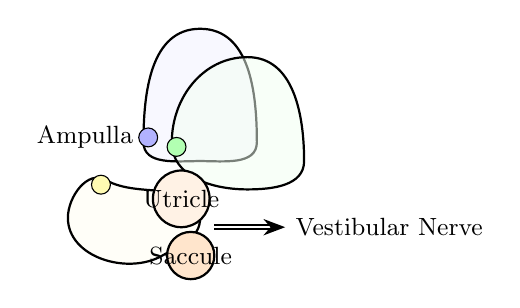
\begin{tikzpicture}[scale=1.2, >=Stealth, every node/.style={font=\small}]
    % Semicircular canals (lateral, anterior, posterior)
    % Anterior canal (vertical, sagittal-ish)
    \draw[thick, fill=blue!5!white, fill opacity=0.5] (0,0) to[out=90,in=180] (0.6,1.2) to[out=0,in=90] (1.2,0) to[out=270,in=0] (0.6,-0.2) to[out=180,in=270] (0,0);
    % Posterior canal (vertical, frontal-ish)
    \draw[thick, fill=green!5!white, fill opacity=0.5] (0.3,0) to[out=90,in=180] (1.1,0.9) to[out=0,in=90] (1.7,-0.2) to[out=270,in=0] (1.1,-0.5) to[out=180,in=270] (0.3,0);
    % Lateral canal (horizontal)
    \draw[thick, fill=yellow!5!white, fill opacity=0.5] (-0.4,-0.4) to[out=150,in=90] (-0.8,-0.8) to[out=270,in=210] (0.2,-1.2) to[out=30,in=270] (0.6,-0.8) to[out=90,in=330] (-0.4,-0.4);
    
    % Utricle and Saccule
    \draw[thick, fill=orange!10!white] (0.4,-0.6) circle (0.3) node {Utricle};
    \draw[thick, fill=orange!20!white] (0.5,-1.2) circle (0.25) node {Saccule};
    
    % Ampullae (swollen parts at base of canals)
    \draw[fill=blue!30!white] (0.05,0.05) circle (0.1) node[left=2pt] {Ampulla};
    \draw[fill=green!30!white] (0.35,-0.05) circle (0.1);
    \draw[fill=yellow!30!white] (-0.45,-0.45) circle (0.1);

    % Connect to nerve
    \draw[double, ->, thick] (0.75,-0.9) -- (1.5,-0.9) node[right] {Vestibular Nerve};

    % Labels
    
ode[above] at (0.6,1.2) {Anterior Canal};
    
ode[above right] at (1.1,0.9) {Posterior Canal};
    
ode[left] at (-0.8,-0.8) {Lateral Canal};
  \end{tikzpicture}
  \end{center}

  \item With the help of a suitable example, elucidate the food capturing mechanism associated with filter feeding.\pts{6}
\end{parts}

\pagebreak
\medskip


\noindent   \textbf{Question 3.} Answer the following parts:

\begin{parts}
  \item Describe the structure and functions of a nephron, giving emphasis on the counter-current exchange mechanism.\pts{6}

  
\begin{center}
  
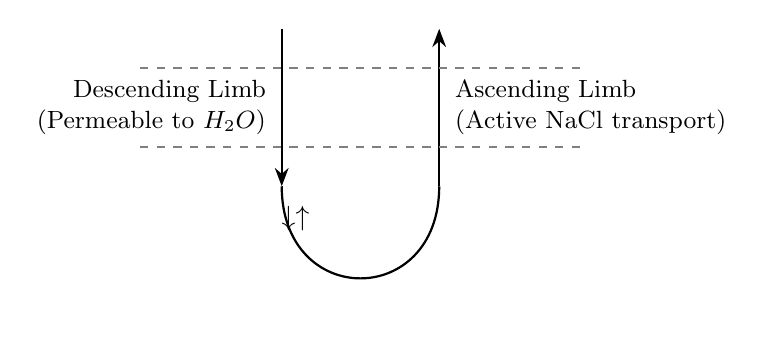
\begin{tikzpicture}[scale=1.0, >=Stealth, every node/.style={font=\small}]
    % Descending Limb (moves down)
    \draw[thick, ->] (0,2.5) -- (0,0.5) node[midway, left=2pt, align=right] {Descending Limb\\(Permeable to $H_2O$)};
    % Hairpin turn
    \draw[thick] (0,0.5) to[out=270, in=270, looseness=2] (2.0,0.5);
    % Ascending Limb (moves up)
    \draw[thick, ->] (2.0,0.5) -- (2.0,2.5) node[midway, right=2pt, align=left] {Ascending Limb\\(Active NaCl transport)};
    
    % Interstitial fluid Osmolarity gradient
    \draw[thick, gray, dashed] (-1.8,2.0) -- (3.8,2.0);
    \draw[thick, gray, dashed] (-1.8,1.0) -- (3.8,1.0);
    
    
ode[left, gray] at (-1.8,2.3) {Cortex};
    
ode[left, gray] at (-1.8,1.5) {Outer Medulla};
    
ode[left, gray] at (-1.8,0.5) {Inner Medulla};

    
ode at (-0.4,2.2) {300};
    
ode at (2.4,2.2) {300};
    
    
ode at (-0.4,1.5) {600};
    
ode at (2.4,1.5) {600};

    
ode at (-0.4,0.7) {900};
    
ode at (2.4,0.7) {900};
    
    
ode at (1.0,-0.3) {1200 mOsm/L};
    
    % Flow indicators
    
ode at (-0.3,1.5) {$\downarrow$};
    
ode at (2.3,1.5) {$\uparrow$};
  \end{tikzpicture}
  \end{center}

  \item With the help of an appropriate diagram, explain how birds maintain continuous unidirectional airflow through their lungs.\pts{6}
  
  
\begin{center}
  
\begin{tikzpicture}[scale=1.1, >=Stealth, every node/.style={font=\small}]
    % Nodes
    
ode[draw, rounded corners, thick, fill=blue!10, minimum width=2cm, minimum height=1cm, align=center] (post) at (3,0) {Posterior\\Air Sacs};
    
ode[draw, rounded corners, thick, fill=orange!10, minimum width=2.2cm, minimum height=1cm, align=center] (lung) at (0,1) {Lungs\\(Gas Exchange)};
    
ode[draw, rounded corners, thick, fill=red!10, minimum width=2cm, minimum height=1cm, align=center] (ant) at (-3,0) {Anterior\\Air Sacs};
    
    % Trachea (Inlet/Outlet)
    
ode (trachea) at (0,-1.5) [draw, fill=gray!10, rounded corners] {Trachea / Outside};

    % Flow arrows
    \draw[->, thick, blue, line width=1.2pt] (trachea) to[out=45, in=270] node[right, pos=0.6] {Inspiration} (post);
    \draw[->, thick, blue, line width=1.2pt] (post) to[out=135, in=0] (lung);
    \draw[->, thick, red, line width=1.2pt] (lung) to[out=180, in=45] (ant);
    \draw[->, thick, red, line width=1.2pt] (ant) to[out=270, in=135] node[left, pos=0.4] {Expiration} (trachea);
  \end{tikzpicture}
  \end{center}
\end{parts}

\medskip


\noindent   \textbf{Question 4.} Write short notes on any two of the following:\pts{$6  \times 2 = 12$}

\begin{parts}
  \item Cranial nerves
  \item Photoreception in rod cells
  \item Mechanism of parthenogenesis in honeybees
\end{parts}

\vfill
\rule{\linewidth}{0.4pt}

\begin{center}\small
\href{https://bhu-exam.vercel.app/}{Click Here}\\[4pt]\href{https://me-aryan.vercel.app/}{Click Here}\\[4pt]\href{https://quashan-me.vercel.app/}{Click Here}
\end{center}

\end{document}
